% Test fixture: injected into main.tex by tests/run_tests.py.
% Segments written as [[...]] are Latin-script text. For pdfLaTeX the
% runner wraps them in \en{...}; for XeLaTeX/LuaLaTeX they are left bare,
% which is exactly what a student would type.
\chapter{Ακραίες Περιπτώσεις: [[Machine Learning]] \& Ελληνικά}
\InitialCharacter{Μ}ικτό κείμενο: χρησιμοποιήσαμε [[Machine Learning]] και
[[Python 3.12]] για το [[project]], π.χ.\ το [[PyTorch]] και το [[scikit-learn]].
Τι είναι το [[Deep Learning]]; Μια ερώτηση με ελληνικό ερωτηματικό.
Άνω τελεία: ναι· σωστά. Ελληνικό ερωτηματικό ως χαρακτήρας: γιατί;

Δύσκολοι χαρακτήρες: αϊδόνι, προϊόν, ΐ, ΰ, Ευρώπη, «εισαγωγικά», ‘μονά’,
παύλα --- και ενωτικό -- , αποσιωπητικά\dots{} τελικό σίγμα: λόγος.
Κεφαλαία με τόνους: Άλφα Έψιλον Ήτα Ιώτα Όμικρον Ύψιλον Ωμέγα.
Παλιό στυλ με \en{(Peer-to-Peer systems)} συνεχίζει να δουλεύει.

\section{[[Related Work]]}
Αναφορές: \cite{goossens93}, \cite{greekbook} και \cite{LiArTs13}.
Υποσημείωση\footnote{Σημείωση με [[English text]] μέσα.} στο κείμενο.
Κώδικας μέσα στη γραμμή: \src{int main()} και ανάποδη κάθετος \bkslash.
Πολύ μεγάλη λέξη: [[Supercalifragilisticexpialidocious]] και σύνδεσμος
\url{https://www.ece.ntua.gr/el/undergraduate/courses?x=1&y=2}.
Ευρετήριο: \indexGR{Σημασιολογικός Ιστός}Σημασιολογικός Ιστός και
\indexEN{Semantic Web}[[Semantic Web]].

\section{Μαθηματικά}
Εξίσωση με ελληνικά γράμματα $\alpha + \beta = \gamma$ και κείμενο στα
μαθηματικά $x \geq 0 \text{ για κάθε } x$:
\begin{align}
	E &= m c^2 \label{eq:emc} \\
	\Delta x \, \Delta p &\geq \frac{\hbar}{2}
\end{align}
Η εξίσωση~\eqref{eq:emc} και ο Πίνακας~\ref{tab:mixed}.

\section{Σχήματα με [[TikZ]]}
Το ελληνικό ερωτηματικό κάνει το ; ενεργό, οπότε δοκιμάζουμε διαδρομές:
\begin{center}
\begin{tikzpicture}
	\draw[thick] (0,0) -- (2,0) -- (1,1.5) -- cycle;
	\node at (1,0.5) {Τρίγωνο};
	\node[below] at (1,0) {[[Triangle]]};
\end{tikzpicture}
\end{center}

\section{Πίνακες και Εικόνες}
\begin{table}[h]
	\centering
	\begin{tabular}{|l|l|}
		\hline
		Ελληνικά & [[English]] \\ \hline
		Μάθηση   & [[Learning]] \\ \hline
	\end{tabular}
	\caption{Μικτός πίνακας [[mixed table]]}
	\label{tab:mixed}
\end{table}
\begin{illustration}[h]
	\centering
	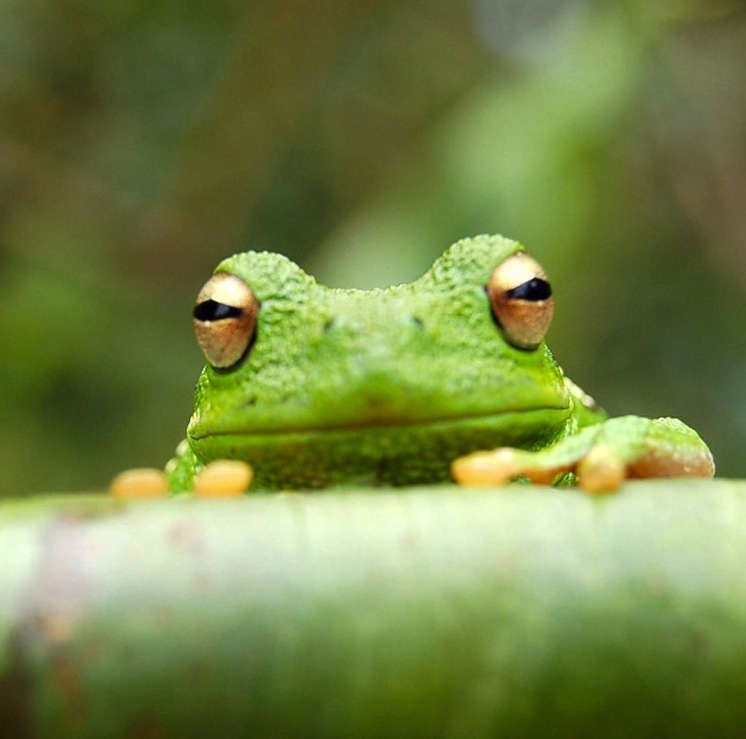
\includegraphics[width=2cm]{figures/frog.jpg}
	\caption{Εικόνα με [[frog]]}
\end{illustration}

\section{Κώδικας}
\begin{lstlisting}[language=Python, basicstyle=\ttfamily\small]
# σχόλιο στα ελληνικά
def hello(name):
    print("Γειά σου", name)  # comment
\end{lstlisting}

\begin{algorithm}[h]
\caption{Αλγόριθμος [[Test]]}
\begin{algorithmic}[1]
	\For{$i \gets 1, n$}
		\If{$i > 0$}
			\State $s \gets s + i$
		\EndIf
	\EndFor
	\State \Return $s$
\end{algorithmic}
\end{algorithm}
